% ----- formatovani dokumentu -----------------------------------------------
\documentclass[12pt,a4paper,titlepage,final]{report}
\usepackage[utf8]{inputenc}
\usepackage[T1, IL2]{fontenc}
\usepackage{graphicx}
\usepackage{epstopdf}
\usepackage[margin=2cm]{caption}
\usepackage[top=3cm, left=2cm, right=2cm, text={17cm, 24cm}, ignorefoot]{geometry}
\usepackage{color}
\usepackage{url}
\usepackage{setspace}
\singlespacing
\usepackage[square, numbers]{natbib} 
\usepackage{float}
\pagestyle{plain}
\pagenumbering{arabic}
\setcounter{page}{1}
\setcounter{secnumdepth}{-1}
\setlength{\parindent}{1cm}	
\usepackage{natbib}
\usepackage{amsmath}
\usepackage{tocloft}
\usepackage{esvect}
\usepackage{amssymb}
\usepackage{gensymb}
\usepackage{subcaption}
\usepackage[algoruled,boxed,lined,longend]{algorithm2e}


\DeclareMathOperator{\dis}{d}

  \newenvironment{czechalgorithm}[1][htb]
  {\renewcommand{\algorithmcfname}{Algoritmus}% Update algorithm name
   \begin{algorithm}[#1]%
  }{\end{algorithm}}

% ----- vyberte jazyk -------------------------------------------------------
\usepackage[english,czech]{babel}
%\usepackage[english]{babel}

% ----- dopiste titulky -----------------------------------------------------
\newcommand\Course{Pokročílá počítačová grafika}
\newcommand\WorkTitle{Generování terénu}
\newcommand\AuthorA{Petr Flajšingr}
\newcommand\AuthorAEmail{xflajs00@stud.fit.vutbr.cz}
\newcommand\Faculty{Fakulta Informačních Technologií}
\newcommand\School{Vysoké Učení Technické v Brně}

\usepackage[
pdftitle={\WorkTitle},
pdfauthor={\AuthorA}
bookmarks=true,
colorlinks=true,
breaklinks=true,
urlcolor=blue,
citecolor=blue,
linkcolor=blue,
unicode=true,
]
{hyperref}


% ----- titulni strana ------------------------------------------------------

\begin{document}
	\begin{titlepage}
	\begin{center}
		
\includegraphics[height=5cm]{images/logo.eps}
	\end{center}
	\vfill
	\begin{center}
		\begin{Large}
			\Course\\
		\end{Large}
		\bigskip
		\begin{Huge}
			\WorkTitle\\
		\end{Huge}
	\end{center}
	\vfill
	\begin{center}
		\begin{large}
			\today
		\end{large}
	\end{center}
	\vfill
	\begin{flushleft}
		\begin{large}
			\begin{tabular}{lll}
				Autor: & \AuthorA, & \url{\AuthorAEmail} \\
				& \Faculty \\
				& \School \\
			\end{tabular}
		\end{large}
	\end{flushleft}
\end{titlepage}		

\section{Úvod}
Tato práce se zabývá implementací generování procedurálního terénu na grafické kartě. Generování a vykreslování terénu je implementováno pomocí c++20 a OpenGL. V práci jsou dále popsány další využité metody jako cascaded shadow mapping, level of detail a další.

\section{Generování terénu}
Pro generování terénu existuje mnoho přístupů. Nejpopulárnějším jsou asi výškové mapy, kdy je hodnota šumu přímo přenášena do výškových souřadnic. Jednoduchou implementaci výškových map můžete najít na adrese \url{https://github.com/PetrFlajsingr/TerrainAnimation}. Tento přístup má ale jeden hlavní nedostatek; neumožňuje vykreslovat více vrstev terénu (jeskyně, převisy...). Aby byl schopen můj engine zobrazovat i složitější útvary zvolil jsem algoritmus marching cubes.

\subsection{Marching cubes}
Algoritmus marching cubes pracuje na principu transformace voxelů do polygonální sítě. Pro výpočet je prostor rozdělen na několik malých částí (kostek) a v nich je vytvořeno 0 až 5 trojúhelníku -- podle konfigurace voxelu. Celkový počet možných konfigurací v rámci jedné kostky je 256. Na obrázku \ref{fig:mc} je ukázka několika možných konfigurací.


\begin{figure}[H]
    \centering
    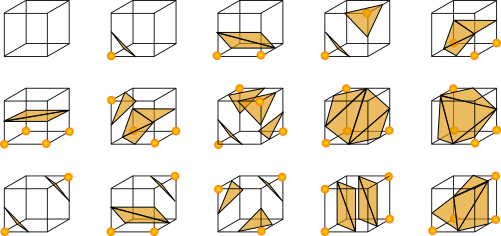
\includegraphics[scale=1]{images/MarchingCubes.png}
    \caption{Ukázka konfigurací}
    \label{fig:mc}
\end{figure}

\subsubsection{Algoritmus generování}
Celé generování probíhá kompletně na grafické kartě. Algoritmus je rozdělen do několika kroků z nichž každý je reprezentován samostatným programem pro GPU. Níže najdete popis generování sítě pro jeden chunk -- tento proces je opakován pro všechny chunky, které je nutné vytvořit.

Prostor je pro každý chunk dělen na oblasti o velikosti 32x32x32 jednotek -- velikost těchto jednotek je určena konfiguračním souborem.

V algoritmu je využíváno look-up tabulek pro konfigurace buněk a vztahy mezi hranami a vrcholy kostek.

\begin{enumerate}
    \item Generování hustoty terénu -- v této fázi jsou do bufferu, který reprezentuje voxely v prostoru, zapsány hodnoty funkce určující rozložení terénu. Hodnoty nižší než 0 reprezentují oblast mimo terén, vyšší než 0 uvnitř terénu a 0 je povrch. Tento krok je realizován pomocí compute shaderů. Funkce pro generování šumu je založena na článku \cite{Backes2018RealTimeMT}.
    \item Streaming markerů pro voxely -- prokaždý voxel je vytvořen flag reprezentující jeho konfiguraci (obrázek \ref{fig:mc}). Konfigurace je určena existencí vertexu na hraně kostky. Jedná se tedy o 8 bitů kde 0 reprezentuje existenci vertexu na dané hraně. V této fázi jsou zahozeny veškeré prázdné voxely, pokud tedy nevygenerujeme žádné hodnoty nemusíme pokračovat dále a můžeme chunk označit jako prázdný. Realizováno pomocí geometry shaderů a transform feedback.
    \item Streaming markerů pro hrany -- snadno můžeme rapidně snížit množství zpracovávaných dat tím, že pro každou kostku budeme zpracovávat pouze hrany jí vlastní, abychom se vyhnuli vícenásobnému generování vertexů na stejné pozici pro různé voxely. Vybereme tedy pouze hrany napojené na nultý vrchol a pro ně vystreamujeme marker pokud se na nich nachází vrchol. Realizováno pomocí geometry shaderů a transform feedback.
    \item Generování vertexů/normál -- pro každý marker z minulého kroku je vygenerován vertex následovně: Pomocí hodnot hustoty terénu ve vrcholech kostky sousedící se zpracovávanou hranou vypočteme finální pozici vertexu (rovnice \ref{eq:vertex}). 

    \begin{equation}\label{eq:vertex}
    v = v_0 + (v_1 - v_0) * \frac{density(v_0)}{abs(density(v_0) - density(v_1))}
    \end{equation}

    Zároveň generujeme normály pro jednotlivé vertexy. Pro výpočet normál je opět využito funkce hustoty. Samplujeme funkci všemi směry čímž získáme její gradient. Po jeho normalizaci dostaneme přesnou normálu povrchu.
    
    Realizováno pomocí vertex shaderů a transform feedback.
    
    \item Ukládání vertex IDs -- jelikož potřebujeme vytvořit element buffer abychom mohli síť vykreslit, je potřebné podniknout několik kroků. Prvním y nich je uložení informací o indexech vertexů. Do bufferu odpovídající velikosti chunku (32x32x32 * počet hran pro voxel (3)) jsou uloženy indexy na odpovídající pozici. Tento krok je prováděn za využítí markerů hranu z kroku 3. Realizováno pomocí vertex shaderů za využití \texttt{gl\_VertexID}.
    
    \item Generování element bufferu -- po přípravě potřebných informací je možné vygenerovat element buffer pro vykreslování. Průchod probíhá podle markerů pro kostky vygenerovaným v kroku 2. Pro každou kostku, která není prázdná, jsou dohledány indexy v bufferu připraveném v předchozím kroku a jsou vystreamovány do výstupního bufferu. Realizováno pomocí geometry shaderů a transform feedback.
\end{enumerate}

Po provedení těchto kroků můžeme použít buffer hustoty pro další chunk a máme připraveny 3 buffery pro vykreslování -- vertexy, normály a elementy. Na obrázku \ref{fig:sphere} je koule vygenerovaná pomocí marching cubes s růžově vyznačenými normálami.

\begin{figure}[H]
    \centering
    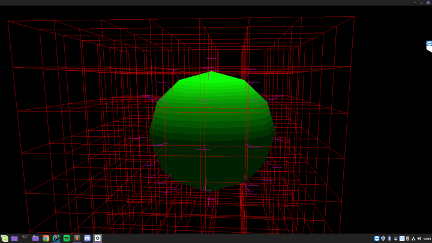
\includegraphics[scale=1]{images/sphere.png}
    \caption{Koule vygenerovaná pomocí marching cubes}
    \label{fig:sphere}
\end{figure}

Jak již bylo naznačeno, nedochází ke generování pouze jednoho chunku, ale velkého množství. Tohle je blíže popsáno v následujících sekcích.

\subsubsection{Nekonečný svět}
Jelikož se jedná o procedurálně generovaný terén tak je vhodné, aby se mohl načítat do nekonečna. Princip funkčnosti je následující. Oblast kolem pozice kamery je rozdělena na 27 podoblastí -- 3x3x3, přičemž středová oblast reprezentuje tu, ve které se nachází kamera. Snad jasněji na obrázku \ref{fig:surr}, kde v levé části došlo k pohybu kamery mezi oblastmi, což vedlo k jejich přeskládání.

\begin{figure}[H]
    \centering
    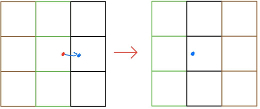
\includegraphics[scale=1]{images/surr.jpg}
    \caption{Přesun okolí podle pohybu kamery (ve 2D pro jednoduchost)}
    \label{fig:surr}
\end{figure}

Každá z těchto oblastí obsahuje pevný počet chunků. Při přesunu je tedy nutné všechny využité chunky ve smazané oblasti recyklovat a chunky v nových oblastech vypočítat. 

Chunky jsou zobrazovány podle vzdálenosti jejich bounding sphere od pozice kamery. Jelikož můžeme vytvořit bounding sphere i kolem celé podoblasti obsahující velké množství chunků, můžeme kontrolovat i jejich vzdálenost a tím ignorovat velké množství vzdálených chunků.

Každý chunk v těchto oblastech také obsahuje informace o tom, jestli byl již spočítán a zda obsahuje nějaké vertexy. Pokud neobsahuje tak je v dalších snímcích ignorován. 

\subsubsection{Level of detail}
Vzhledem k tomu, že chceme zobrazovat terén do větší vzdálenosti, je nutné implementovat level of detail. Pro marching cubes lze řešit jednoduchým způsobem -- můžeme rozdělit chunk na 8 menších chunků při překročení hraniční vzdálenosti vůči nějakému obalujícímu tělesu. Zároveň těchto hranic můžeme určit více a tedy přidat několik úrovní detailu.

V rámci projektu je level of detail pro marching cubes implementován pomocí stromu (z nátury marching cubes vyplývá octree). Každý chunk v sobě obsahuje strom, v němž každá úroveň reprezentuje jednu úroveň LOD. Při přesažení vzdálenosti je chunk rozdělen na menší. Ukázka je na obrázku \ref{fig:lod}. Díky tomuto přístupu můžeme chunk v různých částech rozdělit do různých úrovní LOD.

\begin{figure}[H]
    \centering
    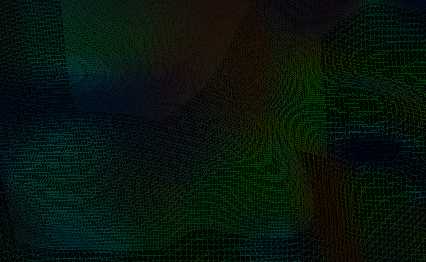
\includegraphics[scale=1]{images/LOD.png}
    \caption{Tři úrovně LOD}
    \label{fig:lod}
\end{figure}

Při procházení stromu pro již existující chunky může nastat několik situací:
\begin{enumerate}
    \item LOD pro větev je stejný -- nic se nemění.
    \item LOD pro větev by měl být snížen (nižší detail) -- recyklujeme chunky použité pro vyšší LOD a spočteme mesh pro úroveň nižší.
    \item LOD pro větev by měl být zvýšen (vyšší detail) -- recyklujeme chunky použité pro nižší LOD a spočteme mesh pro úroveň vyšší.
\end{enumerate}

Tento proces je nutné v každém snímku provést pro všechny neprázdné chunky.

\subsubsection{Detaily implementace}
Vzhledem k tomu, že grafická karta bohužel nemá neomezené množství operační paměti, je nutné omezit množství možných chunků ve scéně. Proto je vytvořen pool chunků, které se střídavě používají. Pokud nejsou ve snímku žádné dostupné tak není možné generovat žádný další terén -- až po recyklaci některých využitých, ať už pomocí LOD nebo vzdálenosti, je možné pokračovat v dalším generování. Zároveň je také omezeno množství chunků, které je možné v každém snímku přidat do fronty výpočtu z důvodu udržení snesitelného FPS.

\section{Vykreslování}
Krom níže zmíněných technik je použito např. View frustum culling. Jedná se ale o základní techniky, které tu nebudu popisovat. 

\subsection{Osvětlení}
Osvětlení je řešeno podle Phongova modelu\footnote{\url{https://en.wikipedia.org/wiki/Phong_reflection_model}}. Jelikož vykreslovaná oblast je poměrně velká je ignorována pozice světla a je použito pouze jeho směru. Na obrázku \ref{fig:light} je vidět vliv osvětlovacího modelu.

\begin{figure}[H]
    \centering
    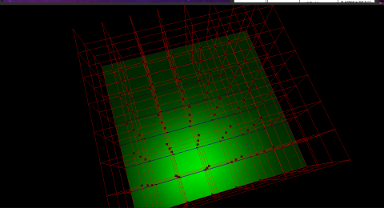
\includegraphics[scale=1]{images/light.png}
    \caption{Ukázka osvětlení}
    \label{fig:light}
\end{figure}

\subsection{Stíny}
Jelikož terén obsahuje velké množství polygonů na velkém prostoru zvolil jsem shadow mapping jako metodu pro tvorbu stínů.

\subsubsection{Shadow mapping}
Shadow mapping funguje na principu vykreslení hloubkové mapy scény z pohledu světla a následném využití této mapy při vykreslování, kdy pokud je fragment dále od světla než hodnota uložená v stínové mapě, je ve stínu. 

\begin{figure}[H]
    \centering
    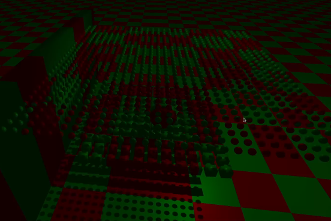
\includegraphics[scale=1]{images/shadow_map.png}
    \caption{Stíny pomocí shadow mapping}
    \label{fig:sm}
\end{figure}

Jelikož při samplování textury a vykreslení stínů vznikají chyby, je nutné je nějak kompenzovat. Prvním problémem jsou okraje stínů, které mohou být "hranaté". To lze vyřešit aplikováním jednoduchého blur kernelu nad texturu, což rozmaže okraje. 

Dalším problémem je "sebe stínění". Opět problém, který lze vyřešit přidáním tzv. "bias", což je hodnota odečítaná od vzdálenosti objektu od světla. Tím efektivně posuneme fragment blíže ke světlu a nedochází k tomuto jevu.

Pro terén samotný je ale tento přístup nedostatečný. Pokud bychom chtěli pokrýt dostatečně velkou oblast, měly by stíny velmi malé rozlišení a docházelo by ke grafickým glitchům.

\subsubsection{Cascaded shadow mapping}
Jedná se o rozšíření shadow mapping. Namísto pevně dané oblasti pro stínovou mapu dělíme view frustum kamery do několika oblastí (obrázek \ref{fig:casc}). Pro každou z těchto oblastí vytvoříme ortogonální projekční matici a vykreslíme do ní stínovou mapu scény. Scéna musí být opakovaně vykreslena tolikrát kolik máme kaskád.

\begin{figure}[H]
    \centering
    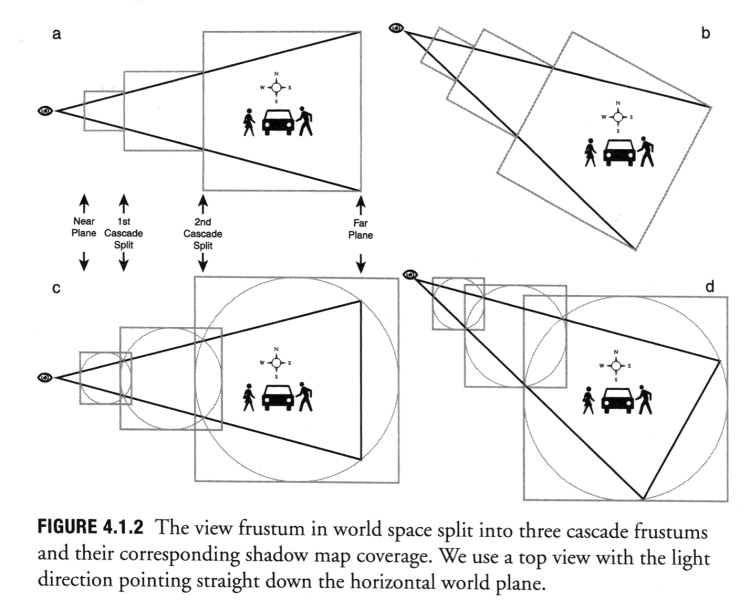
\includegraphics[scale=1.5]{images/cascades.png}
    \caption{Dělba view frusta na kaskády, zdroj: \url{https://johanmedestrom.wordpress.com/2016/03/18/opengl-cascaded-shadow-maps/}}
    \label{fig:casc}
\end{figure}

Samotné vykreslování s kaskádami probíhá obdobně jako v obyčejném shadow mapping pouze s tím rozdílem, že vybíráme ze které textury samplujeme na základě vzdálenosti fragmentu od kamery. Na obrázku \ref{fig:csm} jsou barevně vyznačeny oblasti jednotlivých kaskád -- v tomto případě se jedná o 4 kaskády.

\begin{figure}[H]
    \centering
    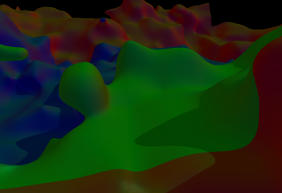
\includegraphics[scale=1]{images/csm.png}
    \caption{Rozdělené scény na kaskády - každá kaskáda je barevně odlišena}
    \label{fig:csm}
\end{figure}

\subsection{Texturování terénu}
Jelikož k terénu není možné vytvořit texturovací koordináty jsou naše možnosti značně omezeny. Jednou možností je aplikace procedurální textury. Ukázka tohoto přístupu je na obrázku \ref{fig:sm}.

Alternativním přístupem je nanášení textur na základě orientace normály povrchu -- trilineární texturování. Můžeme tedy například použít 3 textury, kdy každá z nich je použita pro jeden směr (X, Y, Z). S tímto přístupem můžeme vytvořit poměrně věrohodný povrch. Texturovací koordináty jsou dány pozicí fragmentu v prostoru (tedy například pro osu X se bude jedna o složky y a z) a váha samplované textury je určena délkou normály v dané ose. Výsledek je na obrázku \ref{fig:tex}.

\begin{figure}[H]
    \centering
    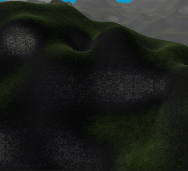
\includegraphics[scale=1]{images/tex.png}
    \caption{Aplikovaná textura}
    \label{fig:tex}
\end{figure}

\subsection{Prostředí}
Pro větší realismus jsem implementoval 2 jednoduché úpravy prostředí.
\subsubsection{Mraky}
Mraky jsou vykreslovány pomocí mapování normál ze zdrojového šumu. Pro každý fragment je samplován šum pro získání jeho gradientu, ze kterého normalizací vytvoříme normálu. Po získání normály vypočteme hodnotu difuzní složky osvětlovacího modelu. Ta je použita jako barevná hodnota a zároveň hodnota alfa kanálu. Jedná se o velmi jednoduchý přístup, ale výsledek je poměrně uspokojivý. Vhodným rozšířením by bylo využití skybox namísto pouze roviny nad kamerou.

\begin{figure}[H]
    \centering
    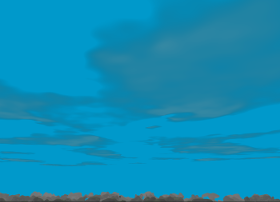
\includegraphics[scale=0.7]{images/clouds.png}
    \caption{Mraky}
    \label{fig:clouds}
\end{figure}

\subsubsection{Mlha}
V projektu je také implementována mlha. Hodnota mlhy pro fragment je dána rovnicí \ref{eq:fog}.

    \begin{equation}\label{eq:fog}
    f = \frac{fog_{end} - vertexCameraDistance}{fog_{end} - fog_{start}}
    \end{equation}

\begin{figure}[H]
    \centering
    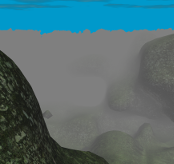
\includegraphics[scale=1]{images/fog.png}
    \caption{Mlha}
    \label{fig:fog}
\end{figure}

\subsubsection{Nedostatky}
Hlavním nedostatkem implementace je rapidní pád FPS při přesunu mezi oblastmi okolí. V tomto případě se musí spočítat velké množství chunků z nově nastavené oblasti, po krátké chvíli se ale počet snímků za sekundu ustálí.

Druhým nedostatkem jsou přechody mezi úrovni level of detail -- tento přechod je vidět na obrázku níže.

\begin{figure}[H]
    \centering
    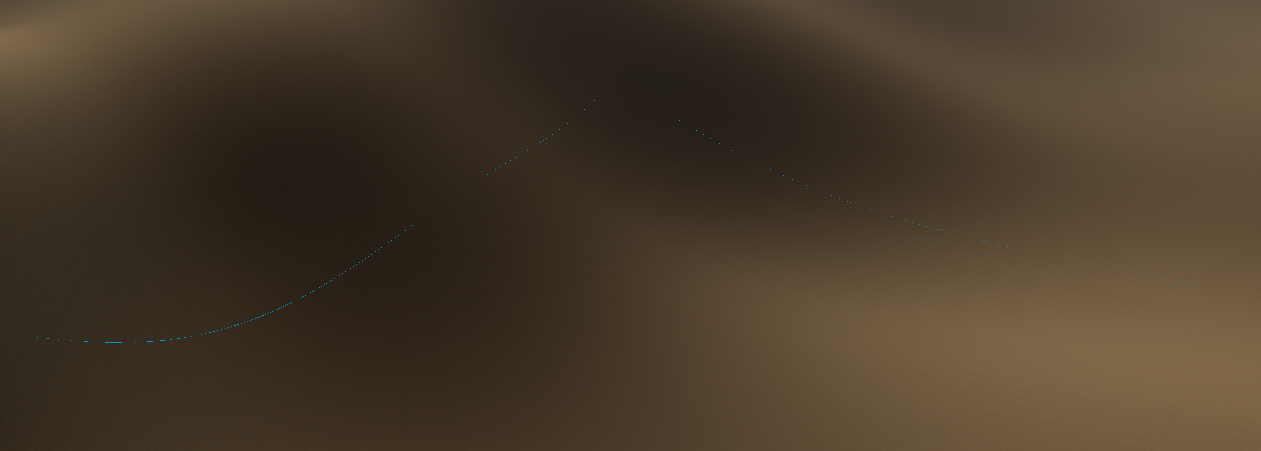
\includegraphics[scale=1]{images/seam.png}
    \caption{Přechod mezi LOD}
    \label{fig:seam}
\end{figure}

\newpage
\section{Použité nástroje a knihovny}
\subsection{Nástroje}
\begin{itemize}
    \item CMake\footnote{\url{https://cmake.org/}}
    \item CLion\footnote{\url{https://www.jetbrains.com/clion/}}
    \item Git\footnote{\url{https://git-scm.com/}}
    \item ClangFormat\footnote{\url{https://clang.llvm.org/docs/ClangFormat.html}}
    \item Perf\footnote{\url{http://man7.org/linux/man-pages/man1/perf.1.html}}
    \item Valgrind\footnote{\url{https://valgrind.org/}}
    \item Google sanitisers\footnote{\url{https://github.com/google/sanitizers}}
\end{itemize}
\subsection{Knihovny}
\begin{itemize}
    \item geGL\footnote{\url{https://github.com/dormon/geGL}}
    \item sdl2cpp\footnote{\url{https://github.com/dormon/SDL2CPP}}
    \item SDL2\footnote{\url{https://www.libsdl.org/}}
    \item \{fmt\}\footnote{\url{https://github.com/fmtlib/fmt}}
    \item FreeType\footnote{\url{https://www.freetype.org/index.html}}
    \item FreeType GL\footnote{\url{https://github.com/rougier/freetype-gl}}
    \item glm\footnote{\url{https://glm.g-truc.net/0.9.9/index.html}}
    \item nlohmann::json\footnote{\url{https://github.com/nlohmann/json}}
    \item observable\footnote{\url{https://github.com/ddinu/observable}}
    \item tinyobjloader\footnote{\url{https://github.com/syoyo/tinyobjloader}}
    \item tinyxml2\footnote{\url{https://github.com/leethomason/tinyxml2}}
\end{itemize}

\section{Struktura projektu}
\begin{itemize}
    \item \texttt{assets}
    \begin{itemize}
        \item \texttt{gui} -- soubory pro uživatelské rozhraní
        \begin{itemize}
            \item \texttt{layout} -- XML definice UI (nedokončeno)
            \item \texttt{fonts} -- *.ttf soubory
        \end{itemize}
            \item \texttt{models} -- OBJ soubory pro modely
        \item \texttt{scenes} -- XML soubory pro definici sceny (částečně dokončeno)
        \item \texttt{textures} -- textury
    \end{itemize}
    \item \texttt{include} -- zdrojové soubory třetích stran
    \item \texttt{rendering}
    \begin{itemize}
        \item \texttt{environment} -- vykreslování okolí (mraky, voda...)
        \item \texttt{marching\_cubes} -- třídy pracující s chunky (LOD, chunk management, nekonečný svět...)
        \item \texttt{models} -- třídy pro načítání a práci s modely
        \item \texttt{shaders} -- GLSL shadery
        \item \texttt{shadow\_maps} -- třídy pro (cascaded) shadow mapping
        \item \texttt{textures} -- třídy pro načítání a debugging textur
    \end{itemize}
    \item \texttt{ui} -- knihovna pro uživatelské rozhraní (více v další sekci)
    \item \texttt{utils} -- utility knihovna (více v další sekci)
\end{itemize}

\newpage
\section{Překlad a ovládání programu}
Pro návod k překladu se prosím obraťte na soubor \texttt{ReadMe.md}, který se nachází u zdrojových souborů. V souboru \texttt{config.md} najdete informace o významu jednotlivých položek konfiguračního souboru.

\begin{figure}[H]
    \centering
    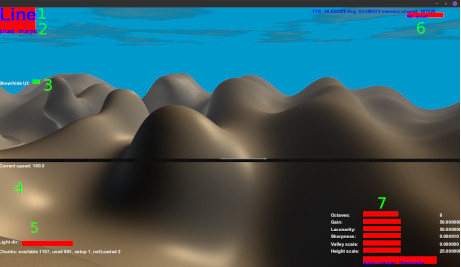
\includegraphics[scale=0.75]{images/controls.jpg}
    \caption{Ovládací prvky programu}
    \label{fig:controls}
\end{figure}

\begin{enumerate}
    \item Tlačítko pro přepnutí mezi polygon/line vykreslováním.
    \item Tlačítko pro zobrazení texture cascaded shadow mapping
    \item Switch pro skrytí/zobrazení UI
    \item Slider pro nastavení rychlosti pohybu kamery
    \item Slider pro nastavení směru světla
    \item Tlačítko pro vypnutí/zapnutí generování nových chunků a LOD
    \item Možnosti nastavení funkce pro generování
    \begin{itemize}
        \item Octaves -- počet oktáv FBM
        \item Gain -- modifikátor amplitudy
        \item Lacunarity -- modifikátor frekvence
        \item Sharpness -- záporné hodnoty přidávají váhu ridge noise, kladné billow noise
        \item Valley scale -- modifikátor velikosti údolí
        \item Height scale -- škálování výšky
        \item Randomize -- náhodně nastaví hodnoty a vygeneruje nově nastavený terén
        \item Apply changes -- vygeneruje nově nastavený terén
    \end{itemize}
\end{enumerate}

Kamera je ovládána pomocí myši a klávesnice. Pro zachycení myši do kamery držte pravé tlačítko myši v libovolné oblasti místo ostatní prvky UI. Kamera udržuje focus dokud nepoužijete jiný UI prvek, poté opět vyžaduje například kliknutí do zmíněné volné oblasti.


\section{Pomocné nástroje vytvořené v rámci projektu}
\subsection{UI}
Vrstva postavená nad sdl2cpp. Zpracovává příchozí eventy z SDL, transformuje je a provádí distpatch pro UI komponenty (implementovány jsou například tlačítka, camera controller, switch, label...). Také podporuje focus systém, viditelnost, překrývání atp.

Využívá knihovny observable pro snadnou práci s měnícími se hodnotami (reaktivní prorgamování).

Pomocí připravených rozhraní lze snadno implementovat nové komponenty. Knihovna nabízí rozhraní pro interakci s myší a klávesnicí. Podporuje i vykreslování textu a využívání různých fontů.

V plánu je rozšířit možnosti definice UI prvků pomocí XML souboru a také změna vykreslování na policy based design kdy bude moct programátor vytvořit vlastní vykreslovací funkce pro komponenty bez nutnosti redefinice jejich chování.

\subsection{Vykreslování modelů}
Pro testovací účely jsem vytvořil rozhraní pro načítání a vykreslování modelů načtených z OBJ souborů. Knihovna podporuje definici jednoduché scény za pomocí XML souboru (scéna na obrázku \ref{fig:sm} byla definována takto). 

\subsection{Utilities}
Utility knihovna obsahující třídy pro geometrii (bounding volumes, view frustum...), výjimky pro error handling s využitím \texttt{std::source\_location}, tree strukturu využitou pro level of detail, nástroje pro meta programování a mnoho dalších (např. obdoba Python \texttt{range} funkce\footnote{\url{https://docs.python.org/3/library/functions.html#func-range}}).

\section{Zhodnocení}
Testováno na AMD Ryzen 5 3600, NVidia GTX 660 Ti. 

\subsection{Rychlost}
Průměrná doba výpočtu jednoho chunku je přibližně 0.5 ms. Pokud bychom tedy pouze generovali, dokážeme vygenerovat až 2000 chunků za sekundu.

Doba výpočtu kontroly viditelnosti a level of detail je odlišná podle vzdálenosti kamery od povrchu a samozřejmě vykreslovací vzdálenosti a mnoha další parametrů. Pro testovací scénu jsou hodnoty následující:

Pokud není žádný chunk rozdělen na vyšší LOD je průměrná doba kontroly přibližně 2.1 ms. V případě rozdělení terénu pomocí LOD se tato doba zvedla o přibližně 40\% na 2.8ms.

Celková průměrná doba vykreslení jednoho snímků s využitím stínů (4 kaskády), osvětlení a okolí (mraky, mlha...) a 800 chunků terénu je v klidovém stavu přibližně 6ms. Při běžném pohybu kamery je doba výrazně delší, přibližně 35ms, kvůli zvýšenému množství kontrol, přepočítávání chunků a jejich případné recyklace. Se zvyšující se rychlostí pohybu se samozřejmě zvyšuje množství změn v každém snímku a tím se zvyšuje doba výpočtu.

Při běžných rychlostech se tedy FPS pohybuje v intervalu 30-60.

\subsection{Paměťová náročnost}
\subsubsection{VRAM}
Pro každý chunk je možné, že využije maximálního množství vertexů, které lze v oblasti vygenerovat. V každém voxelu může vzniknout až 15 vertexů, tedy i 15 normal. Tím je dána maximální možná paměťová náročnost na chunk $max = 32*32*32 * 15 * 2$. Reálně k takovému využití paměti nedojde a většina vypočtených chunků je prázdná či obsahuje maximálně pětinu maximální kapacity. Reálně je tedy náročnost na chunk rovna $\frac{32 * 32 * 32 * 15 * 2}{5} = 196608$ float hodnot, tedy 786432 bytů/chunk. Buffery jsou implementovány se sparse buffer rozšířením pro možnost dynamické práce s pamětí.

Při výpočtech jsou nárazově využity buffery pro uložení hustoty, které mají velikost 413696 bytů/aktuálně počítaný chunk.

Další náročnou položkou jsou textury stínových map. Každá textura má velikost 4096x4096 pixelů s jedním float kanálem, tedy 67108864 bytů/texturu.

Dále samozřejmě případně další modely ve scéně.

\subsubsection{RAM}
Využití operační paměti se, podobně jako VRAM, odvíjí od dohledové vzdálenosti, nastavení LOD atp. Je ale výrazně nižší, než využití VRAM. Nejnáročnější na operační paměť jsou stromové struktury pro LOD, kdy s každou narůstající LOD úrovní vzniká 8x více uzlů stromu než v předchozí úrovni. 

Pro každou oblast musíme udržovat informace o bounding volumes a pozici chunku a další řídící hodnoty. Pro každý uzel stromu tedy zabereme 22 bytů (nepočítaje samotnou stromovou strukturu, která přidává 8 bytů pro každý uzel). Výsledná velikost stromu v paměti pro jeden chunk se třemi LOD úrovněmi je tedy 2190 bytů. V případě, že máme v každé okolní oblasti 10 chunků dostáváme 27000 chunků. Po vynásobení se dostáváme na 59130000 bytů pro celé okolí. 

Aplikace samozřejmě využívá spoustu paměti pro další operace. Za pomocí valgrind jsem zjistil, že využívá cca 300 MB RAM paměti.
\section{Závěr}
Určitě by bylo vhodné nějak snížit paměťovou náročnost na GPU, aby bylo možné generovat rozsáhlejší terén. Dále by bylo vhodné zvolit lepší osvětlovací model a také přesunout kontrolu LOD úrovní na GPU. Na druhou stranu je dle mého generování poměrně svižné, v terénu nedochází ke grafickým glitchům -- krom přechodů mezi LOD -- a s trochou další práce by bylo možné přechody mezi oblastmi výrazně zrychlit.

\nocite{nguyen_2008}
\nocite{cascaded_sm}

\bibliographystyle{plain}
\begin{flushleft}
  \bibliography{references}
\end{flushleft}

\end{document}

